\documentclass[aspectratio=169]{beamer}
\usepackage{graphicx}
\usepackage{pdfpages}
\usepackage[utf8]{inputenc}
\usepackage{natbib}
\usepackage[english]{babel}
\usepackage{amsmath}
\usepackage{graphicx}
\usepackage{booktabs}
\usepackage{tabularx}
\usepackage{array,multirow}
\usepackage{adjustbox}

\usetheme{Dresden}

\title[Mid-term presentation CL Team Lab]
{Mid-term presentation CL Team Lab}
\subtitle{Group 9 Emotion Classification}
\author{Lara Grimminger, Jiwon Kim}
\date{14.06.2021}


%\AtBeginSection[]{
%    \begin{frame}
%        \tableofcontents[currentsection]
%    \end{frame}
%}

\begin{document}

\begin{frame}
\maketitle
\end{frame}

\section{Task Description}


\begin{frame}
\frametitle{Emotion Classification}

\begin{itemize}
\setlength\itemsep{1em}
\item International Survey On Emotion Antecedents And Reactions (ISEAR)
\item Students asked to describe emotional events for 7 emotions including \emph{joy, fear, anger, sadness, disgust, shame}, and \emph{guilt}
\hspace{+5mm}
\begin{itemize}
\setlength\itemsep{0.3em}
\item [$\star$]\emph{joy} - A party I went to last Christmas.
\item [$\star$]\emph{disgust} - An Engineer I know wants war so he can get a job making bombs.

\end{itemize}

\item Supervised Classification Task:\\ Predict correct emotion given a text sequence from the data set

\end{itemize}

\end{frame}


\section{Motivation and Approach}

\begin{frame}
\frametitle{Simple Neural Networks and Data Preprocessing}
\begin{itemize}

\item Neural Network as baseline because it is state-of-the-art architecture
\item Simple 2 and 4-layer Neural Network to understand how architecture works


\end{itemize}
\end{frame}


\section{Method and Experimental Design}
\begin{frame}
\frametitle{Data Preprocessing: tf\_idf and One Hot Encoding}

\begin{itemize}

\item tf-idf = Term frequency (tf) $*$ Inverse document frequency (idf)

\begin{itemize}
\setlength\itemsep{0.4em}
\item [$\star$] $ \text{tf}_{t,d} \: \text{of term t in document d is the number of times t occurs in d} $
\item [$\star$] $\text{df}_t$ is the number of documents that t occurs in

%\item [$\star$] $ \text{idf}_t \: \text{of term t}$ measures the informativeness of the term

\item [$\star$] $ \text{idf}_t \:=\log_{10}\frac{N}{df_t}$, N is the number of documents in the data set
\end{itemize}
\setlength\itemsep{0.8em}
\item One Hot Encoding

\begin{itemize}
\item [$\star$] \emph{joy}$=[1,0,0,0,0,0,0,0]$, \emph{fear}$=[0,1,0,0,0,0,0,0]$, \emph{shame}$=[0,0,1,0,0,0,0,0]$, etc.
\end{itemize}
\end{itemize}
\end{frame}

\begin{frame}
\frametitle{Graphic of 2-Layer Neural Network}

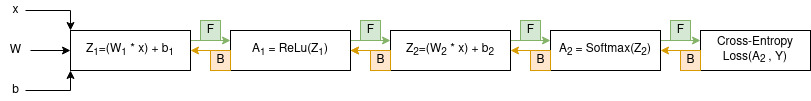
\includegraphics[scale=0.5]{Method_TeamLab.jpg}

\end{frame}

\begin{frame}
\frametitle{Hyperparameters}
\begin{itemize}

\item 2 and 4-layers architecture
\item Tried 5, 10, and 20 epochs
\item Each epoch with $0.01, 0.001, 0.0001, 0.00001$ as learning rates

\end{itemize}
\end{frame}



%\section{Architecture}

%\begin{frame}
%\frametitle{2-Layer Neural Network}
  %# New column type
%\begin{tabular}{m{6.5cm}|m{6.5cm}}                          
%\renewcommand\arraystretch{1.05}
%Forward-propagation & Backward-propagation \\
%\midrule

%input layer: (n\_data, n\_features$=1000$) & Get derivatives\\
%hidden layer:(n\_features=1000, 7) & Reverse steps from forward function  \\
%hidden layer to ReLu function & \\
%output layer: (n\_data, 7) & \\
%output layer to softmax function  & \\
%output to cross-entropy function(loss))&

%\end{tabular}
%\end{center}

%\end{frame}



%\section{Experimental Design}
%\begin{frame}
%\frametitle{Training of the Neural Network}

%\begin{itemize}

%\item Initialization with Kaiming (No exploding or vanishing weights and gradients)
%\item 2 Layers
%\item 1 Epoch
%\item Batchsize of 32
%\item Learning rate of 0.00001

%\end{itemize}

%\end{frame}


\section{Results}

\begin{frame}
\frametitle{Precision, Recall and F$_1$Score}

\begin{table}
\begin{adjustbox}{width=0.35\columnwidth,center}
  \centering
  \setlength{\tabcolsep}{5pt}
  \renewcommand\arraystretch{1.20}
  \begin{tabular}{l l ccc}
  
    \toprule
	 \setlength{\tabcolsep}{8pt}
    Layers & Class &Precision&Recall&F$_1$Score\\
    \cmidrule{1-5}
	\multirow{7}{*}{\rotatebox[origin=c]{90}{\centering 2-layer}}
    &Joy & .13 & 1.0 & .23\\
    &Fear & .00 & .00 & .00\\
    &Shame &  .00 & .00 & .00 \\
    &Disgust & .00 & .00 & .00 \\
    &Guilt & .00 & .00 & .00  \\
    &Anger & .00 & .00 & .00  \\
    &Sadness & .00 & .00 & .00  \\
     \cmidrule{1-5}
    \multirow{7}{*}{\rotatebox[origin=c]{90}{\centering 4-layer}}
   
    &Joy & .13 & 1.0 & .23\\
    &Fear & .00 & .00 & .00\\
    &Shame &  .00 & .00 & .00 \\
    &Disgust & .00 & .00 & .00 \\
    &Guilt & .00 & .00 & .00  \\
    &Anger & .00 & .00 & .00  \\
    &Sadness & .00 & .00 & .00  \\
    \bottomrule
  \end{tabular}
  \end{adjustbox}
\end{table}

\end{frame}

\begin{frame}
\frametitle{Std/mean value of each epoch}
\end{frame}


\section{Next steps}

\begin{frame}
\frametitle{Conclusion and Future Work}

\begin{itemize}
\item Problem: Our baseline predicts the same class regardless of hyperparameters
\setlength\itemsep{0.4em}
\item \emph{Can we improve the performance of the emotion detection method by converting the multi-class classification problem into a binary one? }
%\setlength\itemsep{0.4em}
\begin{itemize}
%\setlength\itemsep{0.4em}
\item [$\star$] Experiment 1:\\ Have one classifier per emotion, e.g. joy vs rest
\item [$\star$] Experiment 2:\\ Have a classifier for a pair of opposite emotions, e.g. joy vs sadness
\end{itemize}


%\begin{itemize}
%\setlength\itemsep{0.4em}
%\item [$\star$] Tackle Curse of Dimensionality with Word Embeddings or PCA
%\item [$\star$] Sequential model of Pytorch
%\end{itemize}
\end{itemize}

%

\end{frame}

\end{document}
